\documentclass[12pt]{article}
\usepackage{graphicx}
\usepackage{mathtools}
\title{Are temperatures of one year significantly correlated with the next year across years in a given location?}
\author{Hannah O'Sullivan h.osullivan18@imperial.ac.uk}
\date{October 2018}

\begin{document}
  \maketitle
  This analysis investigates whether the temperature of one year significantly correlates with that of the next, across years in Key West, Florida. One particular caveat of this analysis is the non-independence of measurements of climatic variables which occur in successive time points in a time series. We calculated the correlation between n-1 pairs of years where n is the total number of years.

  In order to achieve this, the correlation coefficient was first calculated between successive years. We repeated this calculation 10,000 times over a randomly permuted time series. For each randomly permuted year sequence, the correlation coefficient was recalculated.

  The results show a positive correlation between successive years, r = 0.326, p = < 0.001.This suggests that the temperature of one year is significantly correlated with the next year in a given location.

\begin{figure}[ft]
      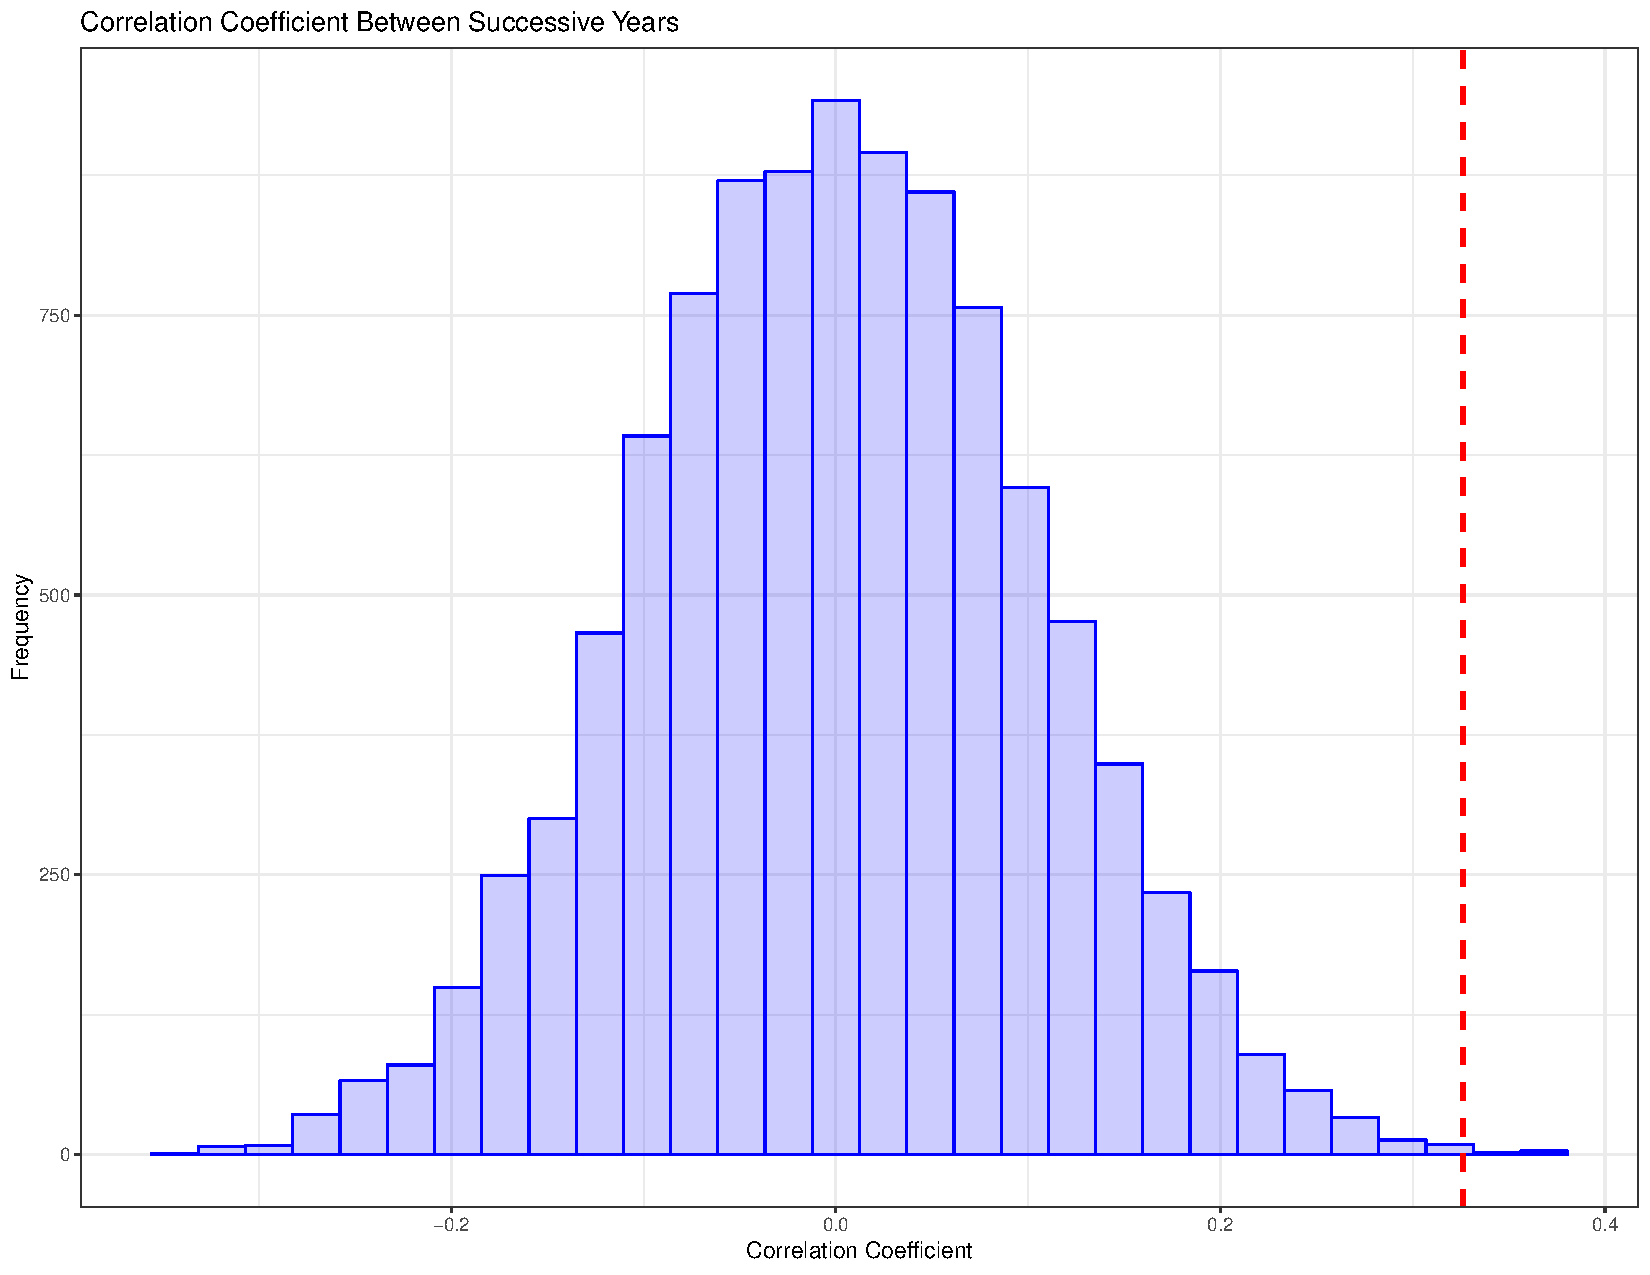
\includegraphics[width = 1\textwidth]{../Data/TAutoCorrPlot.PDF}
      \caption{Figure 1: Distribution of correlation coefficients for each randomly permuted year sequence, showing approximate p-value.}
\end{figure}

\end{document}
